\documentclass[]{article}
\usepackage{amsmath} % flere matematikkommandoer
\usepackage{amssymb}
\usepackage[utf8]{inputenc} % æøå
\usepackage[T1]{fontenc} % mere æøå
\usepackage[danish]{babel} % orddeling
\usepackage{verbatim} % så man kan skrive ren tekst
\usepackage[all]{xy} % den sidste (avancerede) formel i dokumentet
\usepackage{graphicx}
\usepackage{listings}
\usepackage{algorithmic}
\usepackage{algorithm}

\begin{document}

\title{Divide And Conquor}
\maketitle
{\setlength{\parindent}{0 cm}

\section*{Definition}

\textbf{Divide}

Del problemet ind i mindre delproblemer af samme form.\\

\textbf{Conquor}

Løs problemet rekursivt. Hvis problemet er småt nok, løs problemet trivielt.\\

\textbf{Combine}

Sammensæt delløsninger så det større problem bliver løst.

\section*{Eksempel på mergesort}

\newpage
\begin{figure}
  \centering
  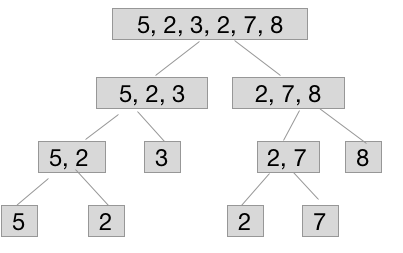
\includegraphics[width=10cm]{graphics/Mergesort Example.png}
  \caption{Rekursionstræet for merge-sort}
  \label{fig:mergeSortTree}
\end{figure}

\newpage

\section*{Mergesort - Proof by induction}
Assume that N is a power of 2\\

$T(N) = 2T(N/2) + N,$ $ \text{for } N > 1, T(1) = 0$

Claim if $T(N)$ satisfies this recurrence then $T(N) = NlgN$

Proof: \\

\textbf{Base case: } $N = 1, T(1) = 0$

\textbf{Inductive Hypothesis: } $T(N) = NlgN$

\textbf{Inductive Step: } $T(2N) = 2Nlg(2N)$

\begin{align}
T(2) &= 2T(N) + 2N\\
	 &= 2NlgN + 2N\\
	 &= 2N(lg(2N) - 1) + 2N\\
	 &= 2Nlg(2N)
\end{align}

\begin{enumerate}
\item{Given}
\item{Inductive Hypothesis}
\item{Algebra}
\item{End of proof (QED)}
\end{enumerate}

}
\end{document}